\documentclass[12pt,a4paper]{report}
\usepackage{amsmath,amsthm,amssymb,graphicx,hyperref,float,mathalpha}
\usepackage[left=1.2in,right=1in,top=1in,bottom=1in]{geometry}
\usepackage[english]{babel}
\usepackage{color}
\usepackage{listings}
\definecolor{mygreen}{rgb}{0,0.6,0}
\definecolor{mygray}{rgb}{0.5,0.5,0.5}
\definecolor{mymauve}{rgb}{0.58,0,0.82}
\definecolor{backcolour}{rgb}{0.95,0.95,0.92}

\lstset{ %
  backgroundcolor=\color{backcolour},   % choose the background color
  numberstyle=\tiny,
  basicstyle=\footnotesize,        % size of fonts used for the code
  breaklines=true,                 % automatic line breaking only at whitespace
  captionpos=b,                    % sets the caption-position to bottom
  commentstyle=\color{mygreen},    % comment style
  escapeinside={\%*}{*)},          % if you want to add LaTeX within your code
  keywordstyle=\color{blue},       % keyword style
  stringstyle=\color{mymauve},     % string literal style
  numbers=left,                    
  numbersep=5pt
}
\usepackage{comment}
\newcommand\tab[1][5mm]{\hspace*{#1}}
\newcommand\taba[1][10mm]{\hspace*{#1}}
\newtheorem{thm}{Teorema}[section]
\newtheorem{lem}[thm]{Lema}
\newtheorem{cor}[thm]{Corolarul}
\newtheorem{prop}[thm]{Propozi\c tia}
\theoremstyle{definition}
\newtheorem{defn}{Defini\c tia}[section]
\theoremstyle{remark}
\newtheorem{rem}{Remarca}[section]
\newtheorem{exmp}{Exemplul}[section]
\begin{document}
\thispagestyle{empty}
\begin{center}
\begin{figure}[h!]
\vspace{-20pt}
\begin{center}

\includegraphics[width=100pt]{FMI-03.png}
\end{center}
\end{figure}

{\large{\bf UNIVERSITATEA DE VEST DIN TIMI\c SOARA

FACULTATEA DE MATEMATIC\u A \c SI INFORMATIC\u A}}

\vspace{65pt}
{\huge {\bf Verification of Neural Networks Competition}}

\vspace{65pt}
\end{center}

\noindent Rafael-Valentin Ban\\
\noindent Cosmin Negureanu\\
\noindent Mihai-Iosif F\^{a}r\c tal\u a \hfill Dr. M\u ad\u alina Era\c scu\\
\noindent Cristina-Larisa Petcu\\
\noindent M\u ad\u alina-Maria Radu\\

\vspace{65pt}
\section*{Abstract}
This benchmark consists of Two-Level Lattice (TLL) NNs, which have been shown to be amenable to fast verification algorithms, for example, FerlezKS22\cite{tll_fast_algorithm} (a fast verification algorithm) can verify whether the output of a given TLL NN always lies within a specified hyper-rectangle whenever its input is constrained to a specified convex polytope (not necessarily a hyper-rectangle).\cite{tll_fast_algorithm} Thus, this benchmark was proposed as a means of comparing TLL-specific verification algorithms with general-purpose NN verification algorithms (i.e. algorithms that can verify arbitrary deep, fully-connected ReLU NNs).\cite{tll_git}
\tableofcontents

\chapter{Description of the dataset}
\tab The networks in this benchmark are a subset of the ones used in Experiment 3 of FerlezKS22\cite{tll_fast_algorithm}. Each of these TLL NNs has n=2 inputs and m=1 output. The architecture of a TLL NN is further specified by two parameters: N, the number of local linear functions, and M, the number of selector sets. This benchmark contains TLLs of sizes N = M = 8, 16, 24, 32, 40, 48, 56, 64, with 30 randomly generated examples of each (the generation procedure is described in Section 6.1.1 of FerlezKS22\cite{tll_fast_algorithm}). At runtime, the specified verification timeout determines how many of these networks are included in the benchmark so as to achieve an overall 6-hour run time; this selection process is deterministic. Finally, a TLL NN has a natural representation using multiple computation paths Figure 1 of FerlezKS22\cite{tll_fast_algorithm}, but many tools are only compatible with fully-connected networks. Hence, the ONNX models in this benchmark implement TLL NNs by "stacking" these computation paths to make a fully connected NN (leading to sparse weight matrices: i.e. with many zero weights and biases). The TLLnet\cite{tll_net} class contains the code necessary to generate these implementations via the exportONNX method.\cite{tll_git}\\
As mentioned before, the data for this benchmark consists of TLLNNs that were used by the authors for a previous study. The original data consists of neural networks of n = 2 and N = M. Thirty examples of N = M = 8, 16, 24, 32, 40, 48, 56 and 64, with each size having a common neuron count from 256 neurons at N = 8 to 163.834 neurons at N = 64. \\

Paragraful 2 este fain....

asdasdsadas

\begin{figure}[H]
\centering
\fbox{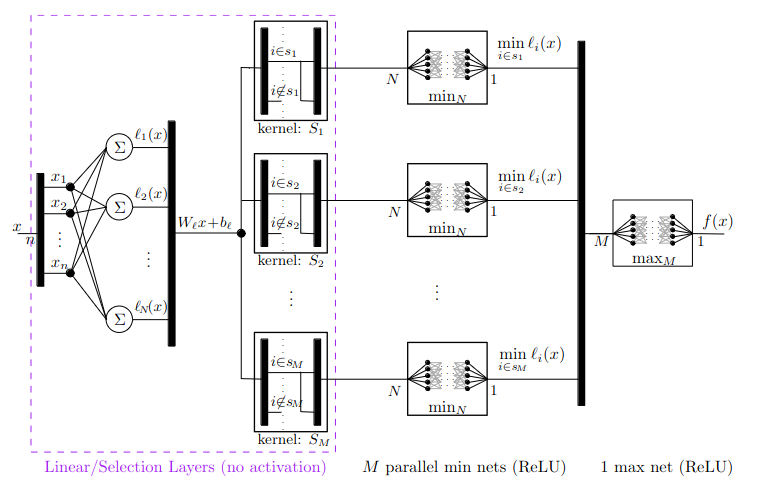
\includegraphics[width=0.8\textwidth]{figure1.png}}
\caption{Figure 1: A TLL NN from \(\mathbb{R}^n\) → \(\mathbb{R}\)\cite{relu_architecture}}
\label{fig:relu_architecture}
\end{figure}
\chapter{Installation of the tools}
\chapter{Run of one tool for the benchmark}
\begin{thebibliography}{1}
\bibitem{tll_git} TLL Verify Bench Repository, "https://github.com/jferlez/TLLVerifyBench"
\bibitem{tll_fast_algorithm} FastBATLLNN: Fast Box Analysis of Two-Level Lattice Neural Networks, "https://dl.acm.org/doi/pdf/10.1145/3501710.3519533"
\bibitem{tll_net} TLLnet, "https://github.com/jferlez/TLLnet"
\bibitem{relu_architecture} James Ferlez and Yasser Shoukry. 2020. AReN: Assured ReLU NN Architecture for
Model Predictive Control of LTI Systems. In Proceedings of the 23rd International
Conference on Hybrid Systems: Computation and Control. Association for Com-
puting Machinery, New York, NY, USA. "https://doi.org/10.1145/3365365.3382213"
\end{thebibliography}
\end{document} 